\documentclass[xcolor={dvipsnames,table}]{beamer}
\usepackage{tikz}                   
\usetikzlibrary{shadows}
\usetheme{Dresden}
\usepackage[utf8]{inputenc}
\usepackage{polski}
\setbeamertemplate{blocks}[rounded][shadow=true]
\setbeamertemplate{footline}[frame number]
\usepackage{booktabs}
%Information to be included in the title page:
\title{Programowanie sprzętu w laboratorium fotoniki}
\author{Paweł Gliwny}
\institute{Instytut Fizyki \\ Politechnika Łódzka}
\date{2017}
 
 
 
\begin{document}
 
\frame{\titlepage}
\begin{frame}
\frametitle{Plan}
\begin{enumerate}
\item Cel pracy
\item Program 
\item Charakterystyki laserów
\end{enumerate}
\end{frame}

\begin{frame}
\frametitle{Cel pracy}
\begin{itemize}
\item Stworzenie programu do wykonywania charakterystyk laserów półprzewodnikowych.
\item Wykonanie przykładowej charakterystyki
\end{itemize}
\end{frame}

\begin{frame}
\frametitle{Układ pomiarowy}
\begin{itemize}
\item Zasilacza diód laserowych firmy Thorlabs model LDC4005 
\begin{figure}
%\hspace{4cm}  \vspace{1cm}
   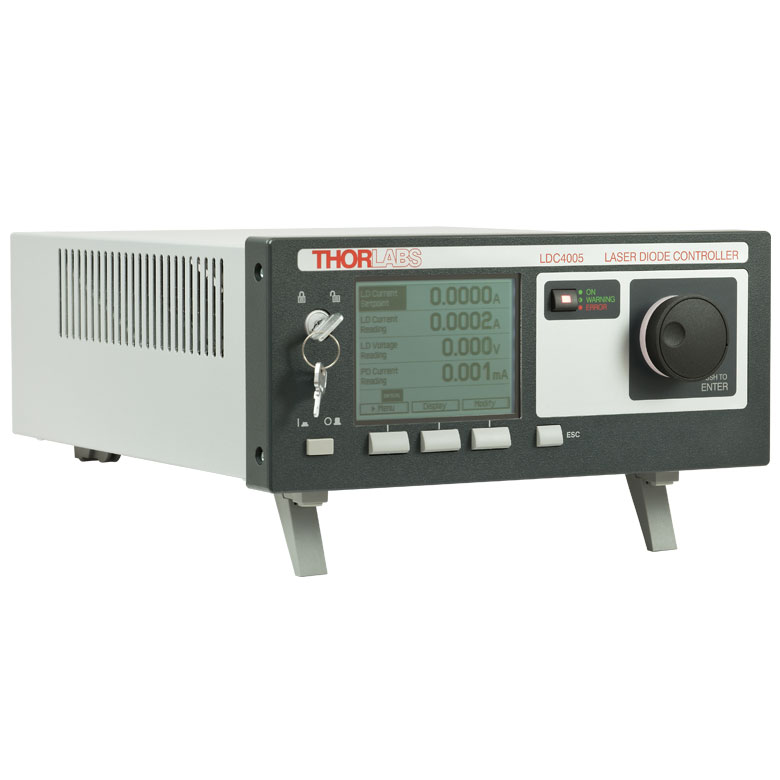
\includegraphics[width=0.35\textwidth,natwidth=69,natheight=87]{ldc4005.jpg}
\end{figure}
\item Miernik mocy firmy Thorlas firmy Thorlabs model PM100
\begin{figure}
%\hspace{4cm}  \vspace{1cm}
   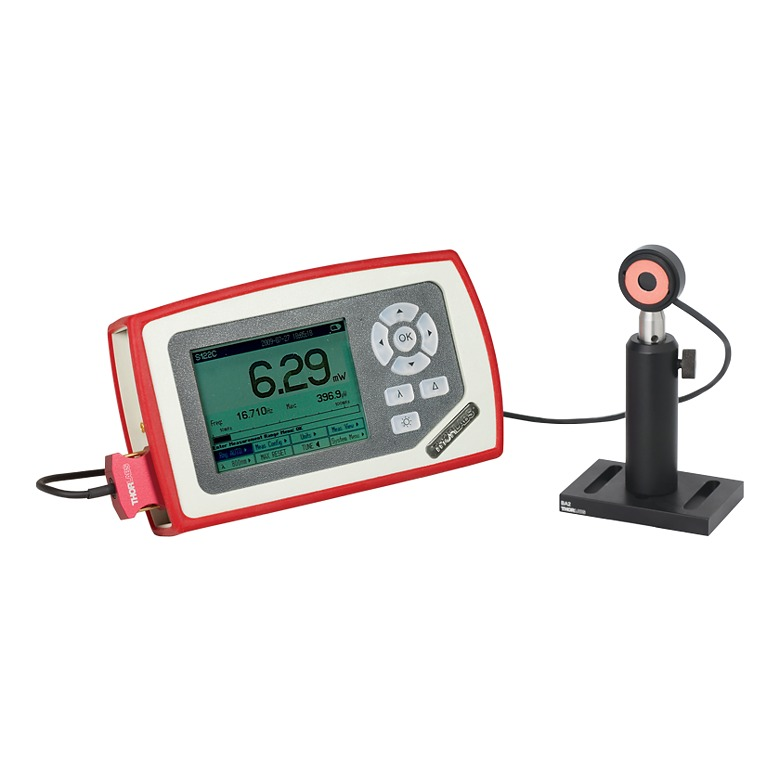
\includegraphics[width=0.35\textwidth,natwidth=69,natheight=87]{pm100.jpg}
\end{figure}
\end{itemize}
\end{frame}


\begin{frame}
\frametitle{Programowane urządzenia pomiarowe}
Electronic test equipment --- są używane w celu przechywywania sygnałów oraz podawanie ich do sprzętu
\end{frame}

\begin{frame}
\frametitle{Komunikacja z urządzenimi}
\begin{itemize}
\item SCPI (ang. Standard Commands for Programmable Instruments) --- język komend do urządzeń pomiarowych.
\item Wywołania systemowe (ang. System call)
\end{itemize}
SCPI + Wywołania systemowe = komunikacja z sprzętem laboratoryjnym
\end{frame}


\end{document}